\let\negmedspace\undefined
\let\negthickspace\undefined
\documentclass[journal]{IEEEtran}
\usepackage[a5paper, margin=10mm, onecolumn]{geometry}
%\usepackage{lmodern} % Ensure lmodern is loaded for pdflatex
\usepackage{tfrupee} % Include tfrupee package

\setlength{\headheight}{1cm} % Set the height of the header box
\setlength{\headsep}{0mm}     % Set the distance between the header box and the top of the text

\usepackage{gvv-book}
\usepackage{gvv}
\usepackage{cite}
\usepackage{amsmath,amssymb,amsfonts,amsthm}
\usepackage{algorithmic}
\usepackage{graphicx}
\usepackage{textcomp}
\usepackage{xcolor}
\usepackage{txfonts}
\usepackage{listings}
\usepackage{enumitem}
\usepackage{mathtools}
\usepackage{gensymb}
\usepackage{comment}
\usepackage[breaklinks=true]{hyperref}
\usepackage{tkz-euclide} 
\usepackage{listings}
% \usepackage{gvv}                                        
\def\inputGnumericTable{}                                 
\usepackage[latin1]{inputenc}                                
\usepackage{color}                                            
\usepackage{array}                                            
\usepackage{longtable}                                       
\usepackage{calc}                                             
\usepackage{multirow}                                         
\usepackage{hhline}                                           
\usepackage{ifthen}                                           
\usepackage{lscape}
\begin{document}

\bibliographystyle{IEEEtran}

\title{9.2.16}
\author{EE25BTECH11054 - S.Harsha Vardhan}
% \maketitle
% \newpage
% \bigskip
\maketitle 
\renewcommand{\thefigure}{\theenumi}
\renewcommand{\thetable}{\theenumi}
\setlength{\intextsep}{10pt} % Space between text and floats

\numberwithin{align}{enumi}
\numberwithin{figure}{enumi}
\renewcommand{\thetable}{\theenumi}
\vspace{-1em}

\textbf{Question 9.2.16}
Find the area of the region bounded by $y = \sqrt{x}$ and $y = x$.

\solution
The given curves are $y^2 = x$ (for $y \ge 0$) and $y = x$.
The matrix form of the parabola $y^2 - x = 0$ is $\vec{x}^\top\mtx{V}\vec{x} + 2\vec{u}^\top\vec{x} + f = 0$, with parameters:
\begin{align}
\mtx{V} = \myvec{0 & 0 \\ 0 & 1}, \quad \vec{u} = \myvec{-1/2 \\ 0}, \quad f = 0. \tag{1}
\end{align}
The parametric form of the line $y=x$ is $\vec{x} = \vec{h} + \kappa\vec{m}$, with parameters:
\begin{align}
\vec{h} = \myvec{0 \\ 0}, \quad \vec{m} = \myvec{1 \\ 1} \tag{2}
\end{align}
The intersection parameter $\kappa$ :
\begin{align}
\kappa_i = \frac{-\vec{m}^\top(\mtx{V}\vec{h} + \vec{u}) \pm \sqrt{[\vec{m}^\top(\mtx{V}\vec{h} + \vec{u})]^2 - g(\vec{h})(\vec{m}^\top\mtx{V}\vec{m})}}{\vec{m}^\top\mtx{V}\vec{m}} \tag{3}
\end{align}
where $g(\vec{h}) = \vec{h}^\top\mtx{V}\vec{h} + 2\vec{u}^\top\vec{h} + f$.
With $\vec{h} = \vec{0}$, we have $g(\vec{h}) = 0$ and $\mtx{V}\vec{h} = \vec{0}$.
The terms for the formula are:
\begin{align}
\vec{m}^\top\mtx{V}\vec{m} &= \myvec{1 & 1} \myvec{0 & 0 \\ 0 & 1} \myvec{1 \\ 1} = 1 \tag{4} \\
\vec{m}^\top(\mtx{V}\vec{h} + \vec{u}) &= \vec{m}^\top\vec{u} = \myvec{1 & 1} \myvec{-1/2 \\ 0} = -1/2 \tag{5}
\end{align}
Substituting into equation (3):
\begin{align}
\kappa_i = \frac{-(-1/2) \pm \sqrt{(-1/2)^2 - 0}}{1} = \frac{1}{2} \pm \frac{1}{2} \tag{6}
\end{align}
The values for $\kappa$ are:
\begin{align}
\kappa_1 = 1, \quad \kappa_2 = 0 \tag{7}
\end{align}
The points of intersection are found by substituting $\kappa_i$ into the line equation:
\begin{align}
\vec{x_1} &= \myvec{0 \\ 0} + 1 \cdot \myvec{1 \\ 1} = \myvec{1 \\ 1} \tag{8} \\
\vec{x_2} &= \myvec{0 \\ 0} + 0 \cdot \myvec{1 \\ 1} = \myvec{0 \\ 0} \tag{9}
\end{align}
The area is given by the integral:
\begin{align}
A &= \int_{0}^{1} (\sqrt{x} - x) \,dx \tag{10} \\
&= \left[ \frac{2}{3}x^{3/2} - \frac{1}{2}x^2 \right]_0^1 \tag{11} \\
&= \left( \frac{2}{3} - \frac{1}{2} \right) - (0) \tag{12} \\
&= \frac{1}{6} \tag{13}
\end{align}
\begin{figure}[h]
    \centering
    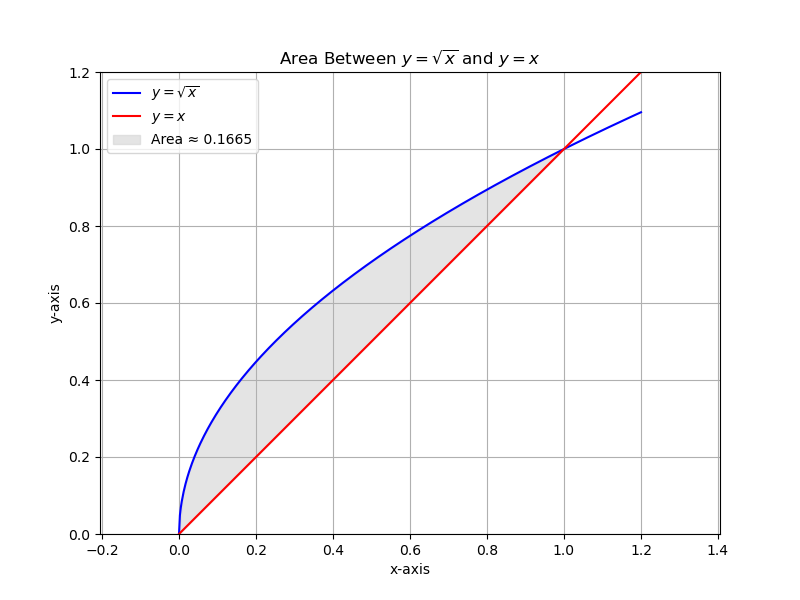
\includegraphics[width=1.1\linewidth]{figs/Figure_9.png}
    \caption{}
    \label{fig:placeholder}
\end{figure}
\end{document}